\documentclass[12pt]{article}
\usepackage[T5]{fontenc}
\usepackage[utf8]{inputenc}
\usepackage[english]{babel}
\usepackage{amsmath, amssymb, bm}
\usepackage{graphicx}
\usepackage[colorlinks=true,
            linkcolor=blue,
            filecolor=magenta,
            urlcolor=cyan,
            citecolor=green,
            bookmarks=true,
            bookmarksopen=true]{hyperref}
\usepackage{enumitem}
\usepackage{geometry}
\geometry{margin=1in}
% \usepackage{listings}
\usepackage{minted}
\usepackage{xcolor}
\usepackage{caption}

\newminted[pythoncode]{python3}{linenos, style=vs_lm, framerule=0.5pt, frame=single, breaklines}

\title{Chapter 15 Report: \\ Modeling Sequential Data Using Recurrent Neural Networks}
\author{Quan Pham}
\date{\today}

\begin{document}

\maketitle
\tableofcontents
\newpage

\section{Abstract}
In this chapter, I studied convolutional neural networks (CNNs) and their application in image classification tasks. CNNs are designed to extract hierarchical features from images, which makes them highly effective for vision-related problems.

\section{Key concepts}
\subsection{Sequential data}

Sequential data, also known as sequence data or sequences, is a type of data that its elements appear in a certain order, with interdependent relationships over time or position. The order of these elements is crucial, as it provide context and structural information that cannot be ignore during analysis. Changing the order can alter or even eliminate the meaning of the entire dataset. 

Sequential data can have different lengths, from short sequences to very long ones. These are some typical examples:
\textbf{Time series:} Daily stock price, sensor data (temperature, humidity), heart rate.
\textbf{Natural language:} Words in a sentence, sentences in a paragraph.
\textbf{Audio:} Voice waveforms, music sequences.
\textbf{Video:} Sequences of frames
\textbf{Biological sequence:} DNA sequences, protein sequences.

\subsection{Categories of sequence modeling}
If either the input or output is a sequence, the modeling task likely falls into one of these categories:
\begin{itemize}
    \item Many-to-one: The input data is a sequence, but the output is a fixed-size vector or scalar, not a sequence.
    \item One-to-many: The input data is in standard format and not a sequence, but the output is a sequence.
    \item Many-to-many: Both the input and output arrays are sequences. This category can be further divided based on whether the input and output are synchronized.
\end{itemize}

\subsection{Recurrent Neural Networks}
A recurrent neural network (RNN) is any network that contains a cycle within its network connections, meaning that the value of some unit is directly, or indirectly, dependent on its own earlier outputs as an input

Computing activation in an RNN is very similar to standard multilayer peerceptrons and other types of feedforward NNs. For the hidden layer, the net input (preactivation), is computed as follows:
\[\bm{z}_h^{(t)} = \bm{W}_{xh}\bm{x}^{(t)} + \bm{W}_{hh}\bm{h}^{(t-1)} + \bm{b}_h\]
Then, the activations of the hidden units at the time step, $t$, are calculated as follows:
\[\bm{h}^{(t)} = \sigma_h(\bm{z}_h^{(t)}) = \sigma_h(\bm{W}_{xh}\bm{x}^{(t)} + \bm{W}_{hh}\bm{h}^{(t-1)} + \bm{b}_h)\]
Once the activations of the hidden units at the current time step are computed, then the activations of the hidden units at the time step are computed, then the activations of the output units will be computed as follows:
\[\bm{o}^{(t)} = \sigma_o(\bm{W}_{ho}\bm{h}^{(t)} + \bm{b}_o)\]

\subsection{Challenges of learning long-range interactions}
Recurrent neural networks (RNNs) are theoretically capable of capturing dependencies across arbitrary sequence lengths. However, in practice, learning long-range interactions is challenging due to issues such as vanishing and exploding gradients during training. When backpropagating errors through many time steps, gradients can shrink exponentially (vanishing) or grow uncontrollably (exploding), making it difficult for the network to learn dependencies that span long intervals.

The vanishing gradient problem causes the network to "forget" information from earlier time steps, limiting its ability to model long-term dependencies. Conversely, exploding gradients can lead to unstable updates and numerical issues. 

% Various techniques have been proposed to address these challenges, including gradient clipping, careful initialization, and specialized architectures such as Long Short-Term Memory (LSTM) and Gated Recurrent Unit (GRU) networks, which introduce gating mechanisms to better preserve and control information flow over long sequences.

\section{Algorithms and Models Studied}
\subsection{Forward pass in convolution layer}
\begin{align*}
Z^{\text{conv}}[:,:,k] &= \sum_{c=1}^{C_{in}} W[:,:,c,k] * X[:,:,c] \\
Z[:,:,k] &= Z^{\text{conv}} + b[k] \\
A[:,:,k] &= \sigma(Z[:,:,k])
\end{align*}

\subsection{Adam optimization}
\textbf{Adam} (Adaptive Moment Estimation) is a widely used optimization algorithm in training neural networks. It combines the advantages of \textbf{AdaGrad} (adaptive learning rates for individual parameters) and \textbf{RMSprop} (using a moving average of squared gradients). Adam is effective due to its ability to adaptively adjust the learning rate for each parameter based on estimates of the first-order moments (mean) and second-order moments (variance) of the gradients.

\subsection*{Basic Steps:}
Given a learning rate $\alpha$, decay rates $\beta_1, \beta_2 \in [0, 1)$, and a small constant $\epsilon$ to prevent division by zero.
\begin{enumerate}
    \item Initialize moment vectors: $m_0 = \mathbf{0}$, $v_0 = \mathbf{0}$.
    \item For each iteration $t = 1, 2, \dots$:
    \begin{itemize}
        \item Compute the gradient $g_t$ of the loss function at time $t$:
        $$g_t = \nabla_\theta J(\theta_{t-1})$$
        \item Update biased first moment estimate (mean of gradients):
        $$m_t = \beta_1 m_{t-1} + (1 - \beta_1) g_t$$
        \item Update biased second moment estimate (mean of squared gradients):
        $$v_t = \beta_2 v_{t-1} + (1 - \beta_2) g_t^2$$
        \item Perform bias correction for the moments (to counteract initial values being zero):
        $$\hat{m}_t = \frac{m_t}{1 - \beta_1^t}$$
        $$\hat{v}_t = \frac{v_t}{1 - \beta_2^t}$$
        \item Update model parameters:
        $$\theta_t = \theta_{t-1} - \alpha \frac{\hat{m}_t}{\sqrt{\hat{v}_t} + \epsilon}$$
    \end{itemize}
\end{enumerate}

\subsection*{Advantages:}
\begin{itemize}
    \item \textbf{Efficiency:} Performs well in practice across various machine learning tasks.
    \item \textbf{Adaptive:} Adjusts the learning rate for each parameter, leading to faster convergence.
    \item \textbf{Ease of Use:} Does not require extensive hyperparameter tuning; default values often yield good results.
\end{itemize}

\subsection{Regularization}
\begin{itemize}
    \item L2 regularization (weight decay) and dropout help prevent overfitting.
    \item Dropout encourages robust feature learning.
\end{itemize}

\subsection{Other Techniques}
\begin{itemize}
    \item \textbf{Data augmentation}: enhances generalization.
    \item \textbf{Global average pooling}: reduces parameters.
\end{itemize}

\subsection{Example models in the book}
\begin{figure}[!h]
    \centering
    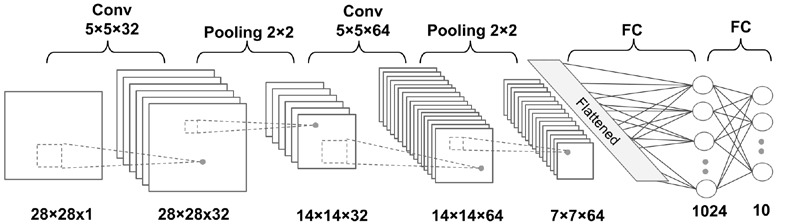
\includegraphics[width=0.9\textwidth]{../figures/deepCNN.jpg}
    \caption{A deep CNN}
\end{figure}


\section{Follow tutorial code in the book}
\subsection{Project one - predicting the sentiment of IMDb reviews}
\subsubsection{IMDb reviews dataset}
The tutorial code loads the IMDb reviews datset using \texttt{torchtext} package. However, \texttt{torchtext} uses \texttt{torchdata} to load data, which doesn't support new python versions. I have to download the dataset from hugging face using pandas.readparquet().

\begin{pythoncode}
splits = {'train': 'plain_text/train-00000-of-00001.parquet', 'test': 'plain_text/test-00000-of-00001.parquet', 'unsupervised': 'plain_text/unsupervised-00000-of-00001.parquet'}
df = pd.read_parquet("hf://datasets/stanfordnlp/imdb/" + splits["train"])

test_dataset = pd.read_parquet("hf://datasets/stanfordnlp/imdb/" + splits["test"])
\end{pythoncode}

Split train dataset to train set and validation set.
\begin{pythoncode}
from sklearn.model_selection import train_test_split
train_dataset, valid_dataset = train_test_split(df, train_size=20000, test_size=5000, random_state=1)
\end{pythoncode}

\subsubsection{Processing the text data}
Tokenization
\begin{pythoncode}
token_counts = Counter()

def tokenizer(text):
    text = re.sub(r'<[^>]*>', '', text)
    emoticons = re.findall(r'(?::|;|=)(?:-)?(?:\)|\(|D|P)', text.lower())
    text = re.sub(r'[\W]+', ' ', text.lower()) +\
        ' '.join(emoticons).replace('-', '')
    tokenized = text.split()
    return tokenized

for i, (text, label) in train_dataset.iterrows():
    tokens = tokenizer(text)
    token_counts.update(tokens)
 
print('Vocab-size:', len(token_counts))
\end{pythoncode}

\begin{verbatim}
Vocab-size: 69353
\end{verbatim}

Vocab
\begin{pythoncode}
from torchtext.vocab import vocab
sorted_by_freq_tuples = sorted(token_counts.items(), key=lambda x: x[1], reverse=True)
ordered_dict = OrderedDict(sorted_by_freq_tuples)
vocab = vocab(ordered_dict)
vocab.insert_token("<pad>", 0)
vocab.insert_token("<unk>", 1)
vocab.set_default_index(1)

print([vocab[token] for token in ['this', 'is', 'an', 'example']])
\end{pythoncode}

collate batch function.
\begin{pythoncode}
device = torch.device('cuda' if torch.cuda.is_available() else 'cpu')

def collate_batch(batch):
    label_list, text_list, lengths = [], [], []
    for _text, _label in batch:
        label_list.append(label_pipeine(_label))
        processed_text = torch.tensor(text_pipeline(_text), dtype=torch.int64)
        text_list.append(processed_text)
        lengths.append(processed_text.size(0))
    label_list = torch.tensor(label_list)
    lengths = torch.tensor(lengths)
    padded_text_list = nn.utils.rnn.pad_sequence(text_list, batch_first=True)
    return padded_text_list.to(device), label_list.to(device), lengths.to(device)
\end{pythoncode}

\subsubsection{Loading data}
Define TabularDataset class, which can return item from dataframe.
\begin{pythoncode}
class TabularDataset(Dataset):
    def __init__(self, dataframe):
        self.dataframe = dataframe
    
    def __len__(self):
        return len(self.dataframe)
    
    def __getitem__(self, idx):
        return self.dataframe.iloc[idx]['text'], self.dataframe.iloc[idx]['label']
\end{pythoncode}

prepare data loaders.
\begin{pythoncode}
batch_size = 32
train_set = TabularDataset(train_dataset)
valid_set = TabularDataset(valid_dataset)
test_set = TabularDataset(test_dataset)

train_dl = DataLoader(train_set, batch_size=batch_size, shuffle=True, collate_fn=collate_batch)
valid_dl = DataLoader(valid_set, batch_size=batch_size, shuffle=False, collate_fn=collate_batch)
test_dl = DataLoader(test_set, batch_size=batch_size, shuffle=False, collate_fn=collate_batch)
\end{pythoncode}

\subsubsection{Train and evaluate model}

\begin{pythoncode}
def train(dataloader, optimizer, loss_fn):
    model.train()
    total_acc, total_loss = 0, 0
    for text_batch, label_batch, lengths in tqdm(dataloader):
        optimizer.zero_grad()
        pred = model(text_batch, lengths)[:, 0]
        loss = loss_fn(pred, label_batch)
        loss.backward()
        optimizer.step()
        total_acc += ((pred >= 0.5).float() == label_batch).float().sum().item()
        total_loss += loss.item() * label_batch.size(0)
    
    return total_acc / len(dataloader.dataset), total_loss / len(dataloader.dataset)

def evaluate(dataloader, loss_fn):
    model.eval()
    total_acc, total_loss = 0, 0

    with torch.no_grad():
        for text_batch, label_batch, lengths in tqdm(dataloader):
            pred = model(text_batch, lengths)[:, 0]
            loss = loss_fn(pred, label_batch)
            total_acc += ((pred >= 0.5).float() == label_batch).float().sum().item()
            total_loss += loss.item() * label_batch.size(0)

    return total_acc / len(dataloader.dataset), total_loss / len(dataloader.dataset)
\end{pythoncode}

\begin{pythoncode}
loss_fn = nn.BCELoss()
optimizer = torch.optim.Adam(model.parameters(), lr=0.001)

num_epochs = 10
torch.manual_seed(1)
print(f'Train model on device {torch.cuda.get_device_name(device)}')
for epoch in range(num_epochs):
    print(f'Epoch {epoch+1}:')
    acc_train, loss_train = train(train_dl, optimizer, loss_fn)
    acc_valid, loss_valid = evaluate(valid_dl, loss_fn)
    print(f'accuracy: {acc_train:.4f} val_accuracy: {acc_valid:.4f}')
\end{pythoncode}

\begin{verbatim}
accuracy: 0.9488 val_accuracy: 0.8466
\end{verbatim}

\begin{pythoncode}
acc_test, _ = evaluate(test_dl, loss_fn)
print(f'test_accuracy: {acc_test:.4f}')
\end{pythoncode}

\begin{verbatim}
test_accuracy: 0.8515
\end{verbatim}

\subsection{Project two - character-level language modeling with Pytorch}

\begin{pythoncode}
vocab_size = len(char_array)
embed_dim = 256
rnn_hidden_size = 512
torch.manual_seed(1)
model = RNN(vocab_size, embed_dim, rnn_hidden_size).to(device)
model
\end{pythoncode}

\begin{pythoncode}
loss_fn = nn.CrossEntropyLoss()
optimizer = torch.optim.Adam(model.parameters(), lr=0.001)

num_epochs = 10000
torch.manual_seed(1)

for epoch in range(num_epochs):
    hidden, cell = model.init_hidden(batch_size)
    seq_batch, target_batch = next(iter(seq_dl))
    seq_batch = seq_batch.to(device)
    target_batch = target_batch.to(device)
    optimizer.zero_grad()
    loss = 0
    for c in range(seq_length):
        pred, hidden, cell = model(seq_batch[:, c], hidden, cell)
        loss += loss_fn(pred, target_batch[:, c])
    loss.backward()
    optimizer.step()
    loss = loss.item()/seq_length
    if epoch % 500 == 0:
        print(f'Epoch {epoch} loss: {loss:.4f}')
\end{pythoncode}

\begin{pythoncode}
def sample(model, starting_str, len_generated_text=500, scale_factor=1.0):
    encoded_input = torch.tensor([char2int[s] for s in starting_str])
    encoded_input = torch.reshape(encoded_input, (1, -1)).to(device)
    generated_str = starting_str
    
    model.eval()
    hidden, cell = model.init_hidden(1)
    for c in range(len(starting_str)-1):
        _, hidden, cell = model(encoded_input[:, c].view(1), hidden, cell)

    last_char = encoded_input[:, -1]
    for i in range(len_generated_text):
        logits, hidden, cell = model(last_char.view(1), hidden, cell)
        logits = torch.squeeze(logits, 0)
        scaled_logits = logits * scale_factor
        m = Categorical(logits=scaled_logits)
        last_char = m.sample()
        generated_str += str(char_array[last_char])

    return generated_str
\end{pythoncode}

\begin{pythoncode}
torch.manual_seed(4)
print(sample(model, starting_str='But what was', scale_factor=2.0))
\end{pythoncode}

Text generated by the model:

"""

\noindent
But what was a complete sure of
the mystery which had been so establiquely. Pencroft, with intending to hoist emotion to all.

Towards six, Cyrus Harding, “whered are the precious verous time to Cyrus Harding’s inhabited; there even intended to survey the cost of the corral.

The six hard later stopped, and then returned to the bay, which were watercourses of our new feet nor their feasts were gazing at the southern part of the ladder--a
right by the fine season whose branches was habitable to remain power 

"""

\section{Pratical exploration with RNNs}
\input{}

\section{Learnings and Challenges}
\subsection{Key Takeaways}

\subsection{Challenges Encountered}

\subsection{Opening Questions}

\section{Conclusion}
\input{contents/conclusion.tex}

% \bibliographystyle{abbrv}
% \bibliography{references}

\end{document}